\setdraft

\begin{frame}{Neural Networks -- Functionality}

% \maketag{un/SUPERVISED} 
\maketag{regression} \maketag{classification}
\maketag{(non)parametric}
\maketag{BLACK-BOX} \maketag{feature selection}

\medskip

\highlight{General idea}
\begin{itemize}
  \item Learn \textbf{composite function} through series of feature 
  transformations, with components distributed over \textbf{neurons}, organized 
  in \textbf{layers}
  \begin{itemize}
    \item Basic neuron operation: 1) affine \textbf{transformation} with 
    weights and bias term, 
    % multiplying inputs with weights (possibly including bias term), 
    2) (nonlinear) \textbf{activation}
    % , applying (nonlinear) function to transformed inputs
    \item \textbf{Arbitrarily complex} combinations of fundamental building 
    blocks
  \end{itemize}
  \item Learning through \textbf{backpropagation}, performing alternating steps:
  \begin{itemize}
    \item \textbf{Forward pass}: predict result with current parameters and 
    compute empirical risk 
    \item \textbf{Backward pass}: update each parameter in proportion to its 
    error contribution $\rightarrow$ gradients
  \end{itemize}
\end{itemize}

\medskip
 
\highlight{Hypothesis space} ~~
$\Hspace = \left\{ \fx: \fx = \tau \circ \phi \circ \sigma^{(h)} \circ
\phi^{(h)} \circ \sigma^{(h - 1)} \circ \phi^{(h - 1)} \circ ... \circ 
\sigma^{(1)} \circ \phi^{(1)} (\xv) \right\}$

\smallskip

\begin{minipage}[b]{0.24\textwidth}
  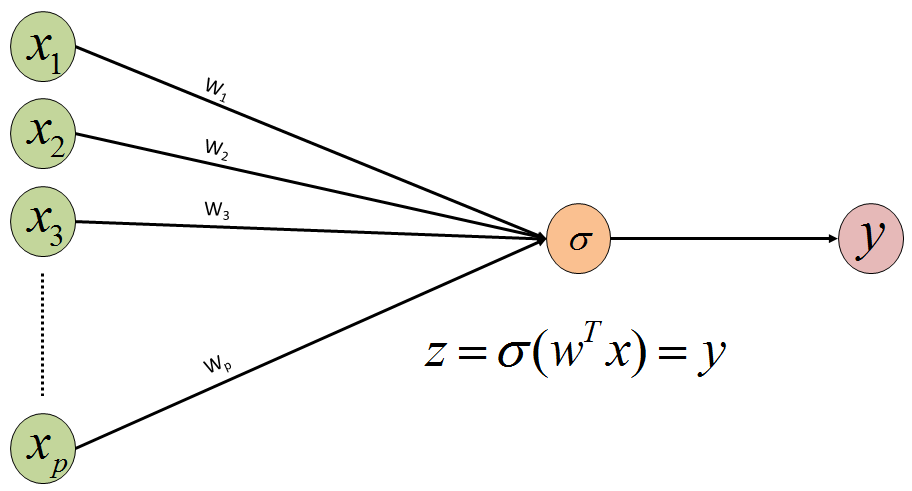
\includegraphics[width=0.9\textwidth]{figure/nn-single-neuron} \\
  \tiny{Single neuron}
\end{minipage}%
\begin{minipage}[b]{0.24\textwidth}
  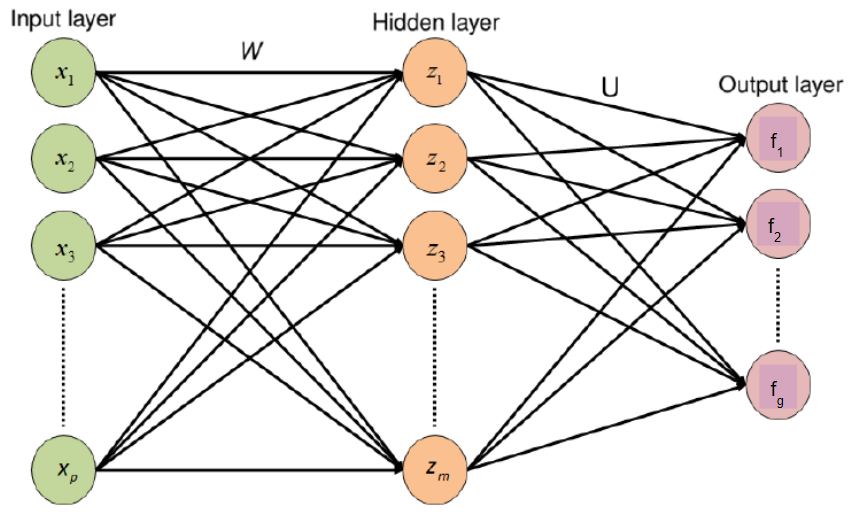
\includegraphics[width=0.9\textwidth]{figure/nn-feedforward} \\
  \tiny{Feedforward network, 1 hidden layer}
\end{minipage}%
\begin{minipage}[b]{0.5\textwidth}
  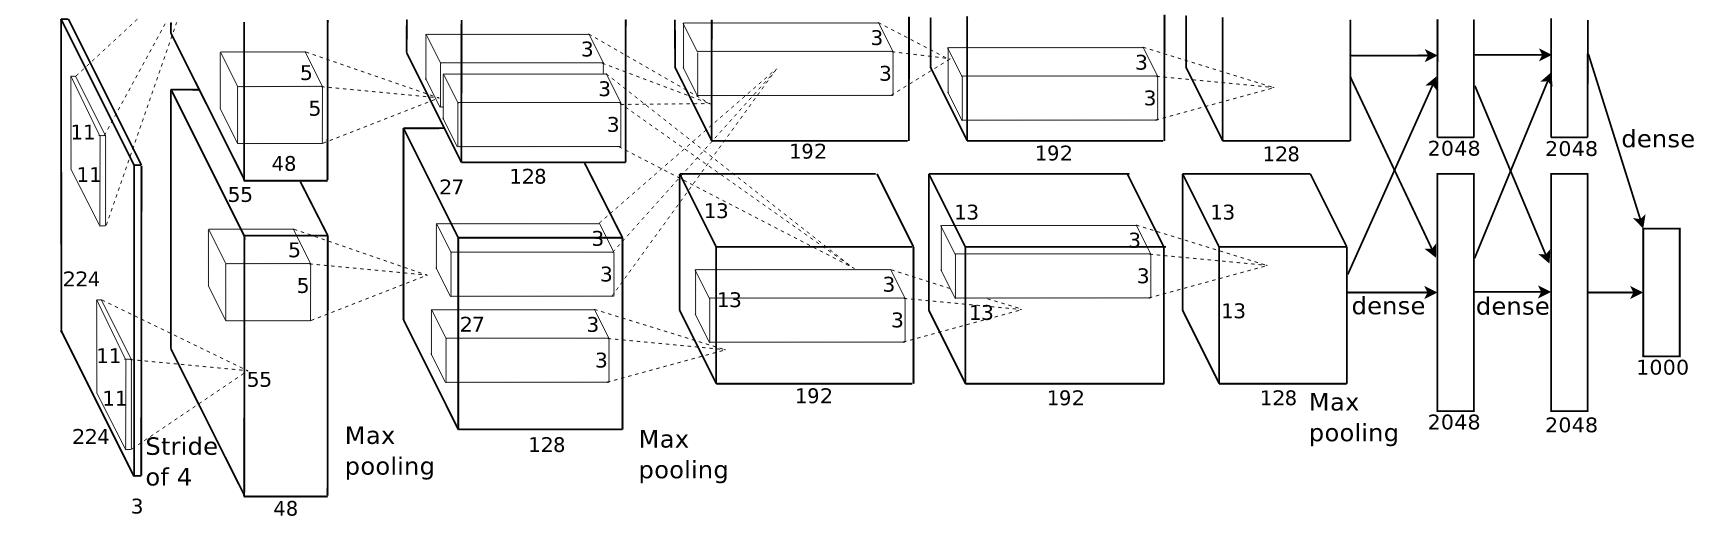
\includegraphics[width=\textwidth]{figure/nn-cnn-1} \\
  \tiny{Convolutional network architecture}
\end{minipage}

\end{frame}

% ------------------------------------------------------------------------------

\begin{frame}{Neural Networks -- Functionality}

\footnotesize

\highlight{Empirical risk} ~~ Any \textbf{differentiable} loss function

\medskip

\highlight{Optimization}

\begin{itemize}
  \item Variety of different optimizers, most based on some form of 
  \textbf{stochastic gradient descent}
  \item Backbone: gradient computation for arbitrary functions via 
  \textbf{computational graphs}
  % \item Crucial role of \textbf{regularization} due to high expressivity of 
  % NNs' hypothesis spaces
\end{itemize}

\medskip

\highlight{NN types} ~~ Large variety of architectures for different purposes
\begin{itemize}
  \item \textbf{Feedforward NNs / multi-layer perceptrons (MLPs):} sequence of 
  \textbf{fully-connected} layers
  \item \textbf{Convolutional NNs (CNNs):} sequence of feature map extractors 
  with spatial awareness $\rightarrow$ images
  \item \textbf{Recurrent NNs (RNNs):} handling of sequential, variable-length 
  information $\rightarrow$ times series, text, audio
  \item Unsupervised: \textbf{autoencoders}, \textbf{generative adversarial 
  networks (GANs)}, \dots
  % \item \textbf{Autoencoders:} learning unsupervised embeddings
  % \item \textbf{Generative adversarial networks (GANs):} learning to generate 
  % artificial samples
\end{itemize}

\highlight{Hyperparameters}

\begin{itemize}
  \item Regarding \textbf{architecture}
  \begin{itemize}
    \item Lots of design choices $\rightarrow$ tuning branch: \textbf{neural 
    architecture search (NAS)}
    \item E.g., network depth, layer types, activation functions, \dots
  \end{itemize}
  \item Regarding \textbf{optimization \& regularization}
  \begin{itemize}
    \item Crucial due to \textbf{overparameterized}, highly \textbf{nonconvex} 
    nature of problem
    \item E.g., weight initialization, choice of optimizer, learning rate, 
    batch size, number of epochs, \dots
  \end{itemize}
\end{itemize}

\medskip

% \highlight{Runtime behavior} ~~ \textcolor{blue}{???}

\end{frame}

% ------------------------------------------------------------------------------

\begin{frame}{Neural Networks -- Pro's \& Con's}

\footnotesize

\begin{columns}[onlytextwidth]
  \begin{column}{0.5\textwidth}
    \highlight{Advantages}
    \footnotesize
    \begin{itemize}
      \positem Able to solve \textbf{complex, non-linear} regression or 
      classification problems
      \positem Therefore, typically very good \textbf{performance}
      \positem Built-in \textbf{feature extraction} - obtained by intermediary
      representations
      \positem Suitable for \textbf{unstructured} data (e. g. image, audio, 
      text data)
      \positem Easy handling of \textbf{high-dimensional} or \textbf{missing} 
      data
      \positem \textbf{Parallelizable} structure
    \end{itemize}
  \end{column}

  \begin{column}{0.5\textwidth}
    \highlight{Disadvantages}
    \footnotesize
    \begin{itemize}
      \negitem Computationally \textbf {expensive} \\
      $\rightarrow$ slow to train and forecast
      \negitem Large \textbf{amounts} of data required 
      \negitem \textbf{Faster-than-linear} scaling of weight matrices with 
      increased network size 
      \negitem Network architecture requiring much \textbf{expertise} in tuning
      \negitem \textbf{Black-box} model -- hard to interpret or explain
      \negitem Tendency towards \textbf{overfitting}
      
    \end{itemize}
  \end{column}
\end{columns}

\vfill

\small

\conclbox{Able to learn extremely complex functions, but computationally 
expensive and hard to get right}

\end{frame}

% ------------------------------------------------------------------------------

\begin{frame}{Neural Networks -- Practical hints}

\highlight{NN regularization}
dropout, batchnorm, lr scheduler, weight decay, ...

\highlight{Optimizers}

batch sizes

% \highlight{Types of neural networks (RNNs, CNNs)}
% 
% \begin{itemize}
%   \item \textbf{Recurrent neural networks (RNNs}: Deep NN that make use of 
%   \textbf{sequential} information with temporal \textbf{dependencies} \\
%   $\rightarrow$ Frequently applied to \textbf{natural language processing}
%   \item \textbf{Convolutional neural networks (CNNs)}: Regularized version of the 
%   fully connected feed-forward NN (where each neuron is connected to all 
%   neurons of the subsequent layer) that abstracts inputs to feature maps via 
%   \textbf{convolution} \\
%   $\rightarrow$ Frequently applied to \textbf{image recognition}
% 
% \end{itemize}
% 
% \medskip
% 
% \highlight{Problem of neural architecture search (NAS)}
% 
% NN are \textbf{not off-the-shelf} methods -- the network architecture needs to 
% be tailored to each problem anew \\
% $\rightarrow$ Automated machine learning attempts to learn architectures

\medskip
 
\highlight{Implementation}

\begin{itemize}
  \item \textbf{R:} packages \texttt{reticulate}, \texttt{neuralnet}
  \item \textbf{Python:} libraries \texttt{PyTorch} and \texttt{PyTorch 
  Lightning}, \texttt{TensorFlow} (high-level API: \texttt{keras})
\end{itemize}

\end{frame}

\undraft